\documentclass[12pt]{beamer}
\usepackage[utf8]{inputenc}
\usepackage[ngerman]{babel}
\usepackage{graphicx}
\usetheme{Dresden}

\usepackage{tikz}
\usepackage{mwe}
\usepackage{pdfpcnotes}

\begin{document}
	\author{Daniel, Fabian, Hauke und Tom (all B.Sc.)}
	\title{Apache Kafka}
	%\subtitle{}
	%\logo{}
	\institute{Modellierung von Informationssystemen\\Department Informatik\\HAW Hamburg}
	\date{01. Dezember 2017}
	%\subject{}
	%\setbeamercovered{transparent}
	\setbeamertemplate{navigation symbols}{}
	
	
\usebackgroundtemplate{		% declare background template 
	\begin{tikzpicture}[remember picture, overlay]
	\node[opacity=1.0, xshift=-3.8cm, yshift=2.25cm, at=(current page.south)] {
		
\includegraphics[scale=0.08]{figure/kafka_diagram.png}};  
	\end{tikzpicture}
}

\begin{frame}[plain]
	\maketitle
\end{frame}

\usebackgroundtemplate{ }    % undeclare background template


\begin{frame}
\section{Konzept}
\frametitle{Was ist Apache Kafka?}
\begin{columns}[T]
	\begin{column}[T]{0.49\textwidth}
		
	\end{column}
	\begin{column}[T]{0.49\textwidth}
		
\end{column}
\end{columns}

\centering
\begin{figure}[h]
	
\includegraphics[scale=0.1]{figure/kafka_diagram.png}
\end{figure}

Apache Kafka ist eine verteilte skalierbare Streaming Plattform.

\pnote{- Beispielkommentar}
\end{frame}


\begin{frame}
\frametitle{Eigenschaften}
Kafka ...
\begin{itemize}
	\item ist ein Message Queuing System
	\item kann Nachrichten speichern
	\item kann Nachrichten verarbeiten
	\item kann all das in Echtzeit
\end{itemize}
\end{frame}

\begin{frame}
\frametitle{Unternehmen und Use Cases}

\begin{tabular}{cl}
	\raisebox{-.25\height}{
\includegraphics[scale=0.2]{figure/linkedin_logo.pdf}} 
		& Operational Metrics\\~\\
	\raisebox{-.25\height}{
\includegraphics[scale=0.2]{figure/cisco_logo.pdf}} 
		& OpenSOC (Security Operations Center)\\~\\
	\raisebox{-.25\height}{
\includegraphics[scale=0.08]{figure/netflix_logo.pdf}} 
		& Real-time monitoring and event-processing pipeline\\~\\
	\raisebox{-.25\height}{
\includegraphics[scale=0.2]{figure/spotify_logo.pdf}} 
		& Log Delivery System\\~\\
	\raisebox{-.25\height}{
\includegraphics[scale=0.1]{figure/twitter_logo.pdf}} 
		& Part of Storm stream processing infrastructure
\end{tabular}

\end{frame}

\begin{frame}
\frametitle{Komponenten}
	\centering
	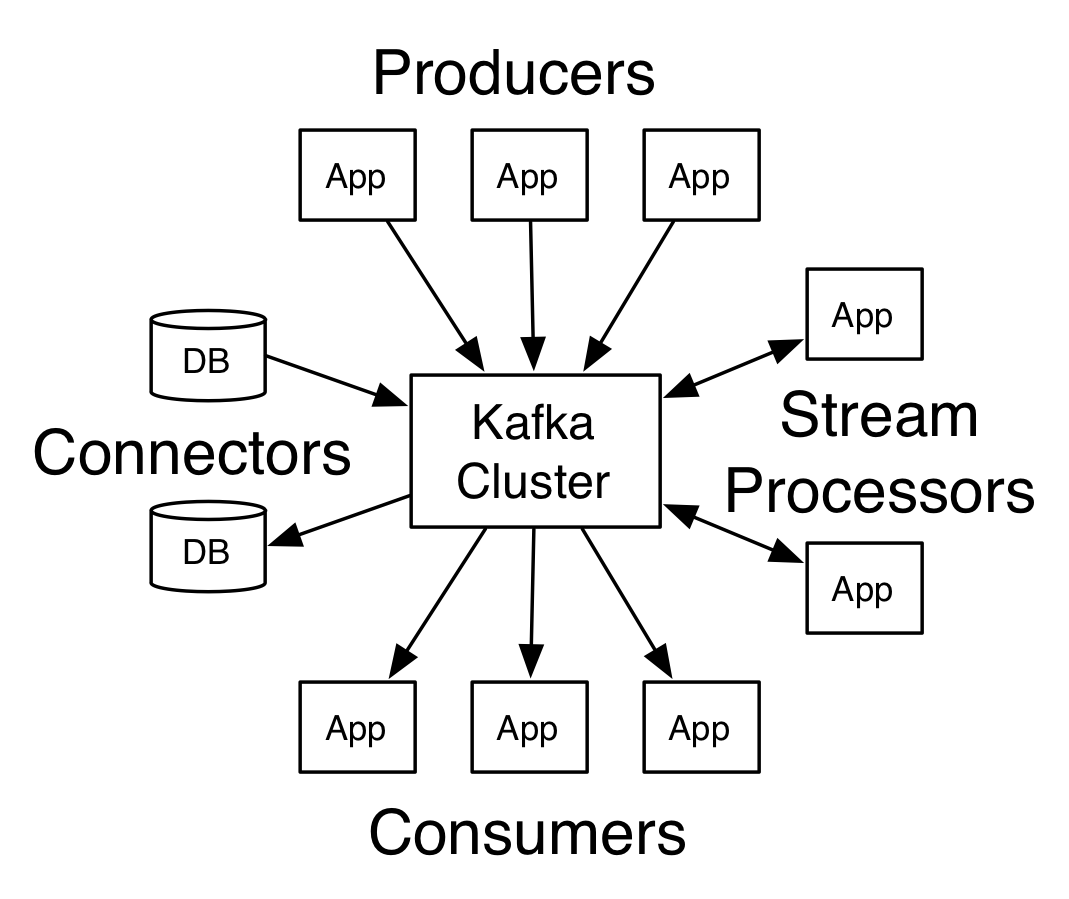
\includegraphics[scale=1.5]{figure/kafka-apis.png}
\end{frame}

\begin{frame}
\frametitle{Queue}
\begin{center}
	\centering
	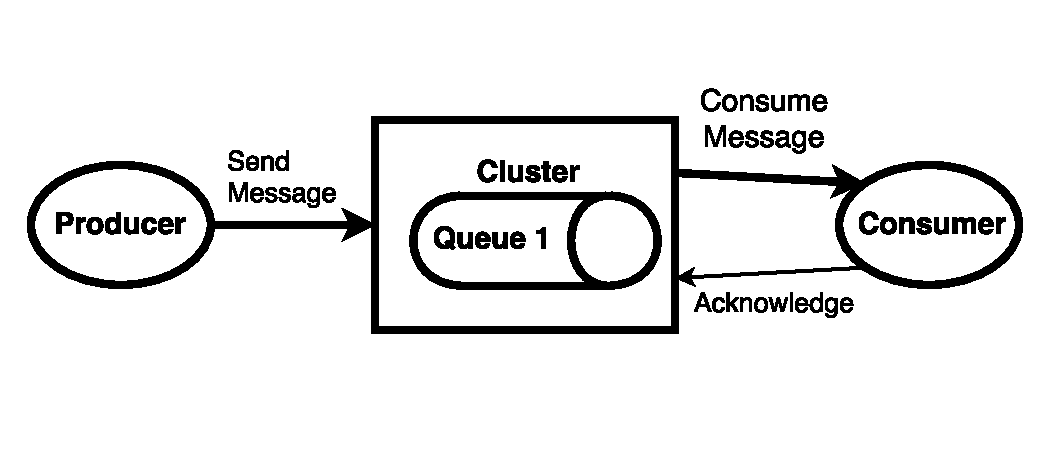
\includegraphics[scale=0.6]{figure/queue_draw.pdf}
\end{center}
\end{frame}

\begin{frame}
\frametitle{Topic}
	\centering
	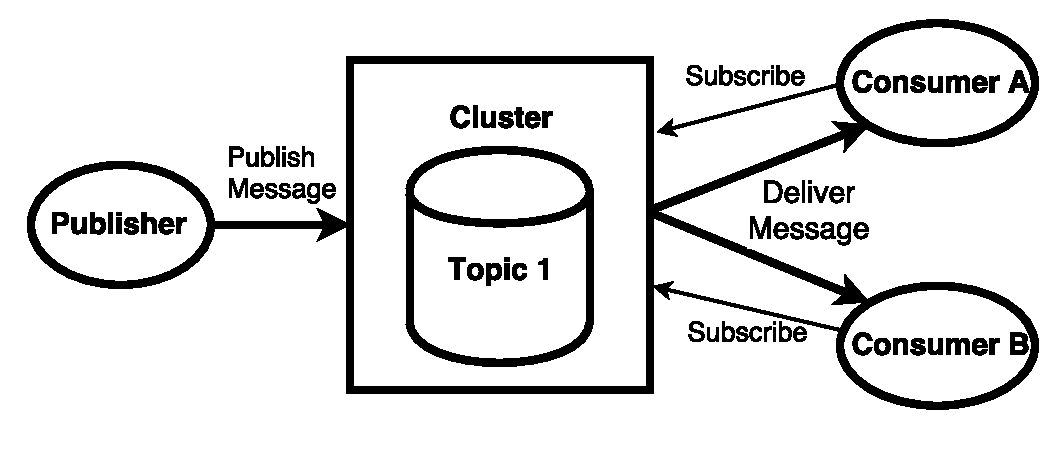
\includegraphics[scale=0.6]{figure/topic_draw.pdf}
\end{frame}

\begin{frame}
\frametitle{Kafka Topics}
\begin{itemize}
	\item Multi-Subscribe ($0$ bis $n$ Consumer)		% Consumergroups - n Anzahl der Partitionen
	\item Kein Push-System
	\item Records in Topics werden persistent gehalten
	\item Topics benötigen eine Cleanup-Policy
		\begin{itemize}
			\item Retention-Time
			\item Retention-Size
			\item Log-Compaction
		\end{itemize}
	\item Topics besitzen Partitionen (partition log)
	\item Guarantees (dazu später mehr)
\end{itemize}
\end{frame}

\begin{frame}
\frametitle{Partitionen}
	\centering
	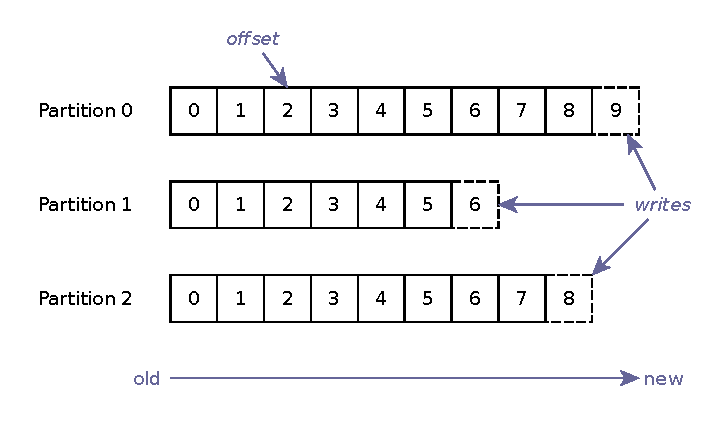
\includegraphics[scale=0.75]{figure/partitioned_log.pdf}
\end{frame}

\begin{frame}
\frametitle{Partitionen}
\centering
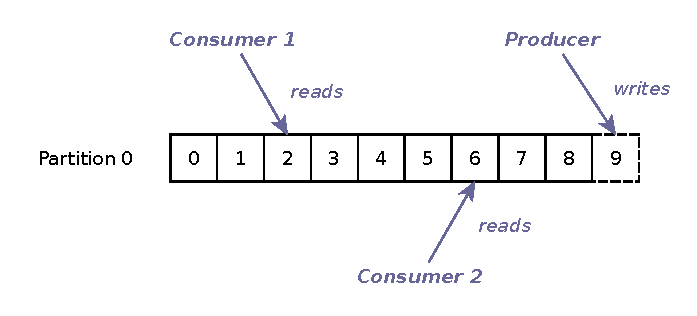
\includegraphics[scale=0.75]{figure/partition.pdf}
\end{frame}

%% Messaging System
\begin{frame}
\frametitle{Kafka als Nachrichtensystem}

Bisher: 
\begin{itemize}
	\item Queueing
	\begin{itemize}
		\item Nachrichten an einen
		\item Nachrichtenverarbeitung skaliert
		\item Nachricht abgerufen = Nachricht weg
	\end{itemize}
	\item Publish-Subscribe
	\begin{itemize}
		\item Nachrichten an alle
		\item Skaliert nicht  			%Jeder bekommt die Nachricht. Daher nicht horizontal skallierbar.
	\end{itemize}
\end{itemize}

\end{frame}

%% Messaging System
\begin{frame}
\frametitle{Kafka als Nachrichtensystem}

\begin{itemize}
	\item Consumer Groups
	\begin{itemize}
		\item Kombiniert Queueing und Publish-Subscribe
		\item Nachrichtenverarbeitung in Gruppen
		\item Mehrere Consumer in einer Gruppe
	\end{itemize}
	\item Vorteile
	\begin{itemize}
		\item Nachrichtenverarbeitung skaliert % Durch Skalierung horizontal Groups und vertical mehrere consumer pro group
	\end{itemize}
	\item Reihenfolge wird eingehalten 
\end{itemize}

\end{frame}

\begin{frame}
\frametitle{Parallelität}

\begin{itemize}
	\item Ordnung 
	\begin{itemize}
		\item Gesichert für alle Consumer Groups
	\end{itemize}
	\item Lastverteilung
		\begin{itemize}
		\item Nachricht 1x pro Consumer Group verarbeitet
	\end{itemize}
\end{itemize}

\end{frame}

%% Storage System
\begin{frame}
\frametitle{Kafka als Datenbank}

\begin{itemize}
	\item Durch Funktionalität bedingt
	\begin{itemize}
		\item Entkopplung sorgt für Speicherbedarf
	\end{itemize}
	\item Daten werden repliziert
	\begin{itemize}
		\item Bestätigungsmechanismen sind vorhanden
		\item Wird erst bestätigt, wenn Replication abgeschlossen ist
	\end{itemize}
\end{itemize}

\end{frame}

\begin{frame}
\frametitle{Kafka als Datenbank - 2}

\begin{itemize}
	\item Performanz bei steigender Datenmenge gleich
	\item Eigenschaften:
	\begin{itemize}
		\item Hohe Performanz
		\item Geringe Latenz %% Für Commit Log Storage
		\item Replikation
		\item Weiterleitung %% Von Nachrichten
	\end{itemize}
\end{itemize}

\end{frame}

\begin{frame}
\frametitle{Kafka für Streams}

\begin{itemize}
	\item Echtzeit Stream-Verarbeitung
	\item Ein Stream Processor:
	\begin{itemize}
		\item Nimmt kontinuierlich Daten aus einem Topic   % Shipments
		\item Bearbeitet die Daten % Preisanpassungen berechnen
		\item Schreibt kontinuierlich Daten in ein Topic % Preisänderungen veröffentlichen
	\end{itemize}
\end{itemize}

\end{frame}


\begin{frame}
\frametitle{Kafka für Streams - 2}

\begin{itemize}
	\item Extra Stream-API wird angeboten
	\begin{itemize}
		\item Ermöglicht komplexere Operationen  % Shipments
		\item Bearbeitet die Daten % Preisanpassungen berechnen
		\item Schreibt kontinuierlich Daten in ein Topic % Preisänderungen veröffentlichen
	\end{itemize}
	\item Kann auch umgehen mit:
	\begin{itemize}
		\item Daten die nicht in Reihenfolge sind  % Shipments
		\item Daten neu verarbeiten wenn sich die Operation ändert % Preisanpassungen berechnen
		\item Status behaftete Operationen sind möglich % Preisänderungen veröffentlichen
	\end{itemize}
\end{itemize}

%The streams API builds on the core primitives Kafka provides: it uses the producer and consumer APIs for input, uses Kafka for stateful storage, and uses the same group mechanism for fault tolerance among the stream processor instances.

\end{frame}

\begin{frame}
\frametitle{Zusammenfassung}

\begin{itemize}
	\item geeignet für:
	\begin{itemize}
		\item   % Shipments
		\item Bearbeitet die Daten % Preisanpassungen berechnen
		\item Schreibt kontinuierlich Daten in ein Topic % Preisänderungen veröffentlichen
	\end{itemize}
\end{itemize}

\end{frame}

% Wie verpacken?
%By combining storage and low-latency subscriptions, streaming applications can treat both past and future data the same way. That is a single application can process historical, stored data but rather than ending when it reaches the last record it can keep processing as future data arrives. This is a generalized notion of stream processing that subsumes batch processing as well as message-driven applications.

%Likewise for streaming data pipelines the combination of subscription to real-time events make it possible to use Kafka for very low-latency pipelines; but the ability to store data reliably make it possible to use it for critical data where the delivery of data must be guaranteed or for integration with offline systems that load data only periodically or may go down for extended periods of time for maintenance. The stream processing facilities make it possible to transform data as it arrives.


\lstdefinestyle{bashstyle}{
    language=bash,
    backgroundcolor = \color{black},
	basicstyle = \color{white}\footnotesize\ttfamily,
	breakatwhitespace=false,         
    breaklines=true,                 
    captionpos=b,                    
    keepspaces=true,                 
    showspaces=false,                
    showstringspaces=false,
    showtabs=false,                  
    tabsize=2,        
    framexleftmargin=6pt,
    framexrightmargin=6pt,
    framextopmargin=6pt,
    framexbottommargin=6pt, 
    frame=tb, 
    framerule=0pt
}
\lstset{style=bashstyle}

\begin{frame}
\section{Tutorial}
\frametitle{Tutorial}
\tableofcontents[currentsection]
\end{frame}

\begin{frame}[fragile]
\subsection{Quickstart}
\frametitle{Quickstart}
\begin{itemize}
\item Download Kafka~\cite{KafkaDownload}
\end{itemize}
\begin{lstlisting}[]
$ tar -xzf kafka_2.11-1.0.0.tgz
$ cd kafka_2.11-1.0.0
\end{lstlisting}

\begin{lstlisting}[]
$ bin/zookeeper-server-start.sh config/zookeeper.properties
$ bin/kafka-server-start.sh config/server.properties
\end{lstlisting}
\end{frame}

\begin{frame}[fragile]
\frametitle{Quickstart}
\begin{lstlisting}[]
$ bin/kafka-topics.sh --create --zookeeper localhost:2181 --replication-factor 1 --partitions 1 --topic test
$ bin/kafka-console-producer.sh --broker-list localhost:9092 --topic test
> This is a message
> This is another message
\end{lstlisting}

\begin{lstlisting}[]
$ bin/kafka-console-consumer.sh --bootstrap-server localhost:9092 --topic test --from-beginning
> This is a message
> This is another message
\end{lstlisting}
\end{frame}

\begin{frame}[fragile]
\subsection{Properties}
\frametitle{Producer Properties}
\begin{table}
{\footnotesize
\begin{tabularx}{\textwidth}{ |X|X|c| } 
\hline 
Name & Beschreibung & Typ \\ \hline \hline
batch-size & Anzahl an Nachrichten die innerhalb eines Batches ins Cluster gepusht werden (asynchrone Kommunikation) & Integer \\ \hline
broker-list/\newline bootstrap.servers & Host- und Portliste zur Verbindung mit dem Cluster & Liste von Strings \\ \hline
message-send-max-retries & Maximale Anzahl an Versuchen das Datum an den Broker zu pushen, bevor der Producer es droped & Integer \\ \hline
topic & Topic unter welches die Daten ins Cluster gepusht werden & String  \\ 
\hline
\end{tabularx}
}
\caption{Beispiele für Producer Properties~\cite{KafkaPropProducer}}
\label{producer_prop}
\end{table}
\begin{center}
\end{center}
\end{frame}

\begin{frame}[fragile]
\frametitle{Consumer Properties}
\begin{table}
{\footnotesize
\begin{tabularx}{\textwidth}{ |X|X|c| } 
\hline 
Name & Beschreibung & Typ \\ \hline \hline
blacklist & Blacklisten von Topics die nicht aboniert werden sollen & Liste von Strings \\ \hline
bootstrap.server/\newline bootstrap.servers & Host und Port zur Verbindung mit dem Cluster & String \\ \hline
from-beginning & Hole die erste Nachricht im Log, sofern der Offset nicht definiert wurde & - \\ \hline
topic & Topic unter welchem die Daten aus dem Cluster geholt werden sollen & String  \\ \hline
whitelist & Whitelisten von Topics die aboniert werden sollen & Liste von Strings \\ 
\hline
\end{tabularx}
}
\caption{Beispiele Consumer Properties~\cite{KafkaPropConsumer}}
\label{consumer_prop}
\end{table}
\begin{center}
\end{center}
\end{frame}

\begin{frame}[fragile]
\frametitle{Weitere Properties}
\begin{itemize}
\item Broker Properties~\cite{KafkaPropBroker}
\item Streams Properties~\cite{KafkaPropStreams}
\item Topic Properties~\cite{KafkaPropTopic}
\item Connect Config Properties~\cite{KafkaPropConnectConfig}
\item AdminClient Properties~\cite{KafkaPropAdminClient}
\end{itemize}
\end{frame}

\begin{frame}[fragile]
\subsection{Kafka Clients}
\frametitle{Kafka Clients}
\begin{itemize}
\item Diverse Clients vorhanden~\cite{KafkaClients}
\begin{itemize}
\item Java, Python, Go, C/C++, .NET, Ruby, ...
\end{itemize}
\item Kafka in Java geschrieben, daher der meiste Support

\end{itemize}
\end{frame}

\begin{frame}[fragile]
\subsection{Twitter App}
\frametitle{Twitter App~\cite{GithubRepo}}
\begin{figure}
\centering
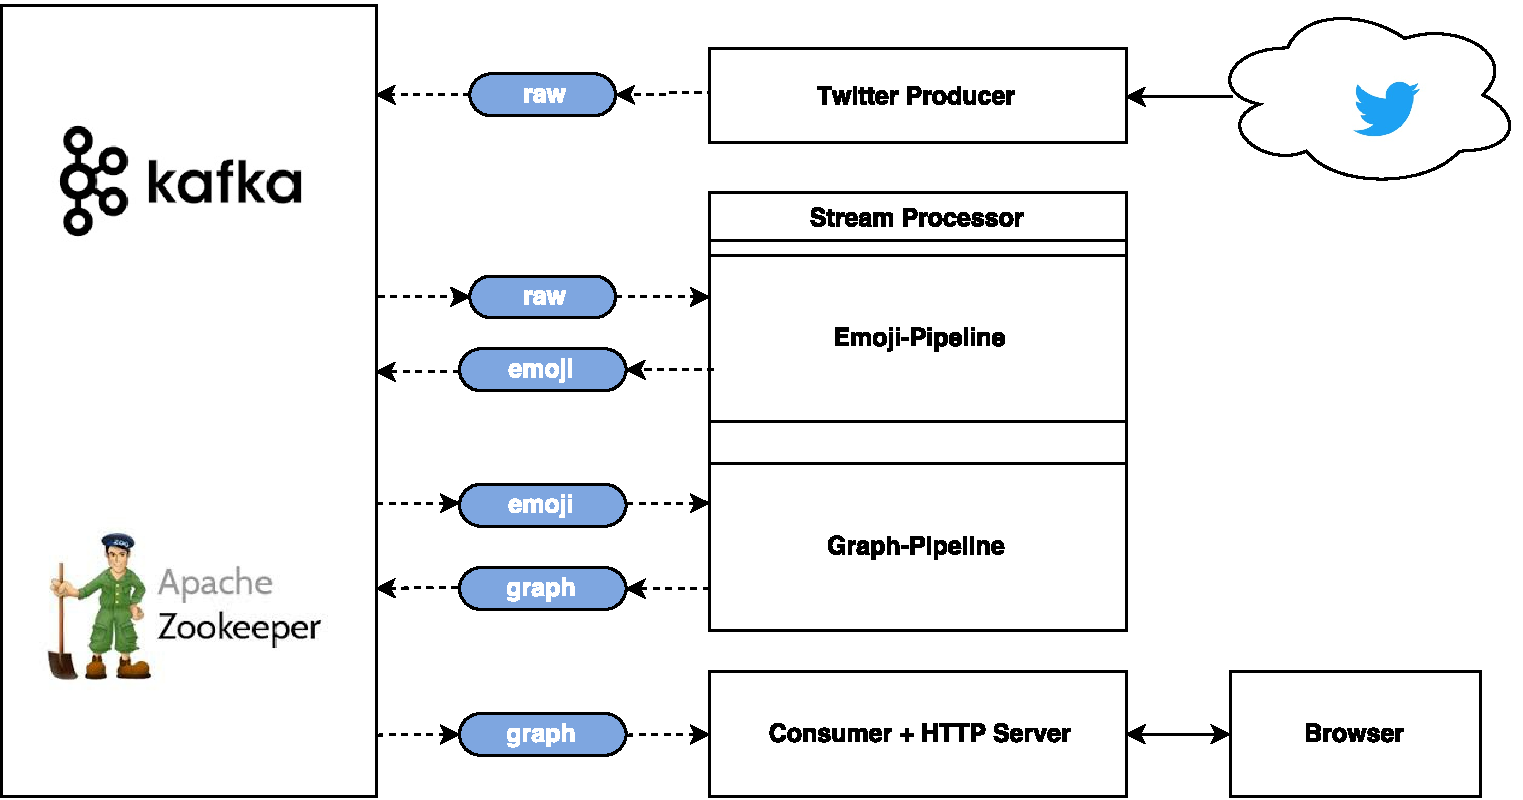
\includegraphics[width=0.95\textwidth]{figure/kafka_tut_diagram.pdf}
\caption{Architektur Twitter App}
\end{figure}
\end{frame}

\definecolor{codegreen}{rgb}{0,0.6,0}
\definecolor{codegray}{rgb}{0.5,0.5,0.5}
\definecolor{codepurple}{rgb}{0.58,0,0.82}
\definecolor{backcolour}{rgb}{0.95,0.95,0.92}
 
\lstdefinestyle{pythonstyle}{
	language=Python,
    basicstyle=\scriptsize\ttfamily,
	backgroundcolor=\color{backcolour},   
    commentstyle=\color{codegreen},
    keywordstyle=\color{magenta},
    numberstyle=\tiny\color{codegray},
    stringstyle=\color{codepurple},
    breakatwhitespace=false,         
    breaklines=true,                 
    captionpos=b,                    
    keepspaces=true,                 
    showspaces=false,                
    showstringspaces=false,
    showtabs=false,                  
    tabsize=2,        
    framexleftmargin=6pt,
    framexrightmargin=6pt,
    framextopmargin=6pt,
    framexbottommargin=6pt, 
    frame=tb, 
    framerule=0pt
}
\lstset{style=pythonstyle}
\begin{frame}[fragile]
\frametitle{Python Producer}
\lstinputlisting[
basicstyle=\scriptsize\ttfamily,
caption=Python Producer]{snippets/snippet-producer.py}
\end{frame}

\begin{frame}[fragile]
\frametitle{Python Processor}
\lstinputlisting[
caption=Python Processor]{snippets/snippet-processor.py}
\end{frame}

\begin{frame}[fragile]
\frametitle{Python Consumer}
\lstinputlisting[
caption=Python Consumer]{snippets/snippet-consumer.py}
\end{frame}

\begin{frame}[fragile]
\frametitle{Screencast}
\begin{center}
\Large{Screencast Demo}
\end{center}
\end{frame}

\begin{frame}
\frametitle{Fragen}
\begin{center}
\Large{Vielen Dank für Eure Aufmerksamkeit!
\\Gibt es Fragen?}
\end{center}
\end{frame}
% \include{section/...}

\end{document}

